We have implemented several use cases to determine the optimal monitoring deployment.
We migrate a virtual network where the target substrate will be supported by physical nodes 1, 2 and 3.
Node 6 is the exfiltration point of the attacker, which means that the attacker will establish a path between node 6 and one of the nodes embedding the virtual network (\ie node 1,2 and/or 3).
In order to make the generation of the MDP states computationally tractable, we set a constant impact performance on all nodes. We set the discount factor of the value iteration algorithm to 0.9, a common value for use cases found in the literature.
We summarize these parameters in Table~\ref{tab:mdp-parameters}.
We compute the optimal policy of each MDP using MDPToolbox~\cite{Chades2014}.

\begin{table}[h]
\centering
\begin{tabular}{|c|c|l|c|c|c|}
\hline
$\alpha$ & \multicolumn{2}{c|}{$\beta$} & Exfiltration point & $c_f$ & $\gamma$ \\ \hline
0.7      & \multicolumn{2}{c|}{3}       & Node 6             & 10    & 0.9      \\ \hline
\multicolumn{6}{|c|}{$V_1=10,V_2=10,V_3=10,V_4=5,V_5=5,V_6=5$}                             \\ \hline
% \multicolumn{6}{|c|}{[10,10,10,5,5,5]}                                          \\ \hline
\multicolumn{6}{|c|}{$\forall j, c_c^j=10$}                             \\ \hline
\multicolumn{6}{|l|}{Physical embedding: Nodes 1 - Node 2 - Node 3}             \\ \hline
\multicolumn{6}{|c|}{Migration order: 1 $\rightarrow$ 2 $\rightarrow$ 3}                              \\ \hline
\end{tabular}
\caption{Use cases parameters}
\label{tab:mdp-parameters}
\end{table}

We propose to evaluate the MDP using three different physical topologies shown in Figure~\ref{fig:mdp-usecase-single}. The first topology is designed to be relatively balanced in terms of connections between nodes. The link between nodes 1 and 4 creates a path so each node can be reached by a single attacker in two steps.

The second topology is full-meshed and is intended to observe the monitoring strategy when the attacker only needs to compromise one node to be successful.

 The last topology defines a central communication point, here node 2. This node should be of prime interest in the solution because it is on the path of every attack in the network.

\begin{figure}[ht]
\centering



\tikzset{every picture/.style={line width=0.75pt}} %set default line width to 0.75pt        

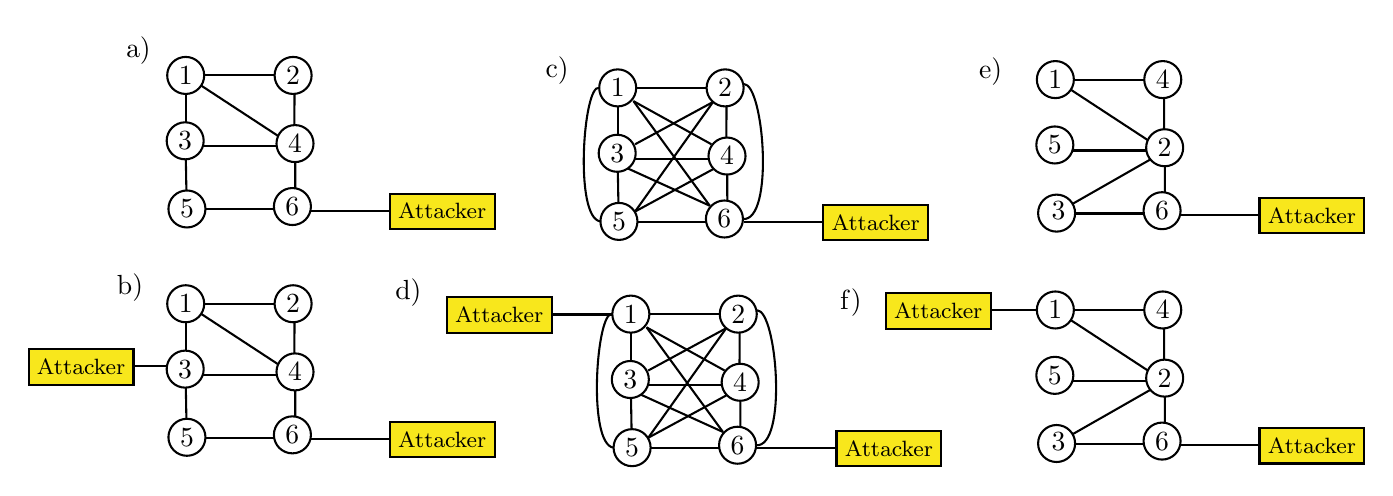
\begin{tikzpicture}[x=0.75pt,y=0.75pt,yscale=-1,xscale=1]
%uncomment if require: \path (0,300); %set diagram left start at 0, and has height of 300

%Straight Lines [id:da21270339539187544] 
\draw    (50.75,166.4) -- (88.67,166.4) ;


%Shape: Rectangle [id:dp19806528063640816] 
\draw  [fill={rgb, 255:red, 248; green, 231; blue, 28 }  ,fill opacity=1 ] (9.2,158.2) -- (59.67,158.2) -- (59.67,175.18) -- (9.2,175.18) -- cycle ;


%Straight Lines [id:da3153834125753151] 
\draw    (137.33,132.22) -- (137.17,163.81) ;


%Straight Lines [id:da7084115546458901] 
\draw    (91.08,200.73) -- (129,200.73) ;


%Straight Lines [id:da9623839826112595] 
\draw    (84.83,136.23) -- (140.58,172.73) ;


%Straight Lines [id:da2909368745777172] 
\draw    (84.83,172.73) -- (85.33,200.55) ;


%Straight Lines [id:da35867881660722734] 
\draw    (137.58,170.73) -- (137.67,202.88) ;


%Shape: Circle [id:dp9939759302306557] 
\draw  [fill={rgb, 255:red, 255; green, 255; blue, 255 }  ,fill opacity=1 ] (75.92,136.23) .. controls (75.92,131.3) and (79.91,127.31) .. (84.83,127.31) .. controls (89.76,127.31) and (93.75,131.3) .. (93.75,136.23) .. controls (93.75,141.15) and (89.76,145.15) .. (84.83,145.15) .. controls (79.91,145.15) and (75.92,141.15) .. (75.92,136.23) -- cycle ;

%Shape: Circle [id:dp34760301125310855] 
\draw  [fill={rgb, 255:red, 255; green, 255; blue, 255 }  ,fill opacity=1 ] (128.58,169.06) .. controls (128.58,164.14) and (132.58,160.15) .. (137.5,160.15) .. controls (142.42,160.15) and (146.42,164.14) .. (146.42,169.06) .. controls (146.42,173.99) and (142.42,177.98) .. (137.5,177.98) .. controls (132.58,177.98) and (128.58,173.99) .. (128.58,169.06) -- cycle ;

%Shape: Circle [id:dp9702116004071654] 
\draw  [fill={rgb, 255:red, 255; green, 255; blue, 255 }  ,fill opacity=1 ] (127.33,199.4) .. controls (127.33,194.47) and (131.33,190.48) .. (136.25,190.48) .. controls (141.17,190.48) and (145.17,194.47) .. (145.17,199.4) .. controls (145.17,204.32) and (141.17,208.31) .. (136.25,208.31) .. controls (131.33,208.31) and (127.33,204.32) .. (127.33,199.4) -- cycle ;

%Straight Lines [id:da8265544446705831] 
\draw    (93.75,136.23) -- (131.67,136.23) ;


%Straight Lines [id:da1435228669726185] 
\draw    (90.75,170.4) -- (128.67,170.4) ;


%Straight Lines [id:da5512583348761163] 
\draw    (84.83,145.15) -- (84.83,163.81) ;


%Shape: Circle [id:dp33954226442737345] 
\draw  [fill={rgb, 255:red, 255; green, 255; blue, 255 }  ,fill opacity=1 ] (76.52,200.56) .. controls (76.52,195.64) and (80.51,191.65) .. (85.43,191.65) .. controls (90.36,191.65) and (94.35,195.64) .. (94.35,200.56) .. controls (94.35,205.49) and (90.36,209.48) .. (85.43,209.48) .. controls (80.51,209.48) and (76.52,205.49) .. (76.52,200.56) -- cycle ;

%Shape: Circle [id:dp027045110799332694] 
\draw  [fill={rgb, 255:red, 255; green, 255; blue, 255 }  ,fill opacity=1 ] (75.67,167.73) .. controls (75.67,162.8) and (79.66,158.81) .. (84.58,158.81) .. controls (89.51,158.81) and (93.5,162.8) .. (93.5,167.73) .. controls (93.5,172.65) and (89.51,176.65) .. (84.58,176.65) .. controls (79.66,176.65) and (75.67,172.65) .. (75.67,167.73) -- cycle ;

%Shape: Circle [id:dp8622510797031577] 
\draw  [fill={rgb, 255:red, 255; green, 255; blue, 255 }  ,fill opacity=1 ] (127.67,136.23) .. controls (127.67,131.3) and (131.66,127.31) .. (136.58,127.31) .. controls (141.51,127.31) and (145.5,131.3) .. (145.5,136.23) .. controls (145.5,141.15) and (141.51,145.15) .. (136.58,145.15) .. controls (131.66,145.15) and (127.67,141.15) .. (127.67,136.23) -- cycle ;

%Straight Lines [id:da8162398929728556] 
\draw    (144.75,201.4) -- (182.67,201.4) ;


%Shape: Rectangle [id:dp15602990655598958] 
\draw  [fill={rgb, 255:red, 248; green, 231; blue, 28 }  ,fill opacity=1 ] (183.2,193.2) -- (233.67,193.2) -- (233.67,210.18) -- (183.2,210.18) -- cycle ;




%Straight Lines [id:da675337569741544] 
\draw    (137.33,22.22) -- (137.17,53.81) ;


%Straight Lines [id:da9770217193149313] 
\draw    (91.08,90.73) -- (129,90.73) ;


%Straight Lines [id:da18857026751215256] 
\draw    (84.83,26.23) -- (140.58,62.73) ;


%Straight Lines [id:da6275844068359788] 
\draw    (84.83,62.73) -- (85.33,90.55) ;


%Straight Lines [id:da3859409733288094] 
\draw    (137.58,60.73) -- (137.67,92.88) ;


%Shape: Circle [id:dp38555186789719464] 
\draw  [fill={rgb, 255:red, 255; green, 255; blue, 255 }  ,fill opacity=1 ] (75.92,26.23) .. controls (75.92,21.3) and (79.91,17.31) .. (84.83,17.31) .. controls (89.76,17.31) and (93.75,21.3) .. (93.75,26.23) .. controls (93.75,31.15) and (89.76,35.15) .. (84.83,35.15) .. controls (79.91,35.15) and (75.92,31.15) .. (75.92,26.23) -- cycle ;

%Shape: Circle [id:dp6614919206504822] 
\draw  [fill={rgb, 255:red, 255; green, 255; blue, 255 }  ,fill opacity=1 ] (128.58,59.06) .. controls (128.58,54.14) and (132.58,50.15) .. (137.5,50.15) .. controls (142.42,50.15) and (146.42,54.14) .. (146.42,59.06) .. controls (146.42,63.99) and (142.42,67.98) .. (137.5,67.98) .. controls (132.58,67.98) and (128.58,63.99) .. (128.58,59.06) -- cycle ;

%Shape: Circle [id:dp4792028510349877] 
\draw  [fill={rgb, 255:red, 255; green, 255; blue, 255 }  ,fill opacity=1 ] (127.33,89.4) .. controls (127.33,84.47) and (131.33,80.48) .. (136.25,80.48) .. controls (141.17,80.48) and (145.17,84.47) .. (145.17,89.4) .. controls (145.17,94.32) and (141.17,98.31) .. (136.25,98.31) .. controls (131.33,98.31) and (127.33,94.32) .. (127.33,89.4) -- cycle ;

%Straight Lines [id:da5503390690988923] 
\draw    (93.75,26.23) -- (131.67,26.23) ;


%Straight Lines [id:da4684291204598492] 
\draw    (90.75,60.4) -- (128.67,60.4) ;


%Straight Lines [id:da14625515615077633] 
\draw    (84.83,35.15) -- (84.83,53.81) ;


%Shape: Circle [id:dp5312971223005962] 
\draw  [fill={rgb, 255:red, 255; green, 255; blue, 255 }  ,fill opacity=1 ] (76.52,90.56) .. controls (76.52,85.64) and (80.51,81.65) .. (85.43,81.65) .. controls (90.36,81.65) and (94.35,85.64) .. (94.35,90.56) .. controls (94.35,95.49) and (90.36,99.48) .. (85.43,99.48) .. controls (80.51,99.48) and (76.52,95.49) .. (76.52,90.56) -- cycle ;

%Shape: Circle [id:dp8123330510491519] 
\draw  [fill={rgb, 255:red, 255; green, 255; blue, 255 }  ,fill opacity=1 ] (75.67,57.73) .. controls (75.67,52.8) and (79.66,48.81) .. (84.58,48.81) .. controls (89.51,48.81) and (93.5,52.8) .. (93.5,57.73) .. controls (93.5,62.65) and (89.51,66.65) .. (84.58,66.65) .. controls (79.66,66.65) and (75.67,62.65) .. (75.67,57.73) -- cycle ;

%Shape: Circle [id:dp008503760549775086] 
\draw  [fill={rgb, 255:red, 255; green, 255; blue, 255 }  ,fill opacity=1 ] (127.67,26.23) .. controls (127.67,21.3) and (131.66,17.31) .. (136.58,17.31) .. controls (141.51,17.31) and (145.5,21.3) .. (145.5,26.23) .. controls (145.5,31.15) and (141.51,35.15) .. (136.58,35.15) .. controls (131.66,35.15) and (127.67,31.15) .. (127.67,26.23) -- cycle ;

%Straight Lines [id:da5256421122460654] 
\draw    (144.75,91.4) -- (182.67,91.4) ;


%Shape: Rectangle [id:dp7797605979818211] 
\draw  [fill={rgb, 255:red, 248; green, 231; blue, 28 }  ,fill opacity=1 ] (183.2,83.2) -- (233.67,83.2) -- (233.67,100.18) -- (183.2,100.18) -- cycle ;




%Straight Lines [id:da22867619419553487] 
\draw    (345.47,28.22) -- (345.31,59.81) ;


%Straight Lines [id:da7366629057200433] 
\draw    (299.22,96.73) -- (337.14,96.73) ;


%Straight Lines [id:da5560609381608291] 
\draw    (292.97,68.73) -- (293.47,96.55) ;


%Straight Lines [id:da4739025620423759] 
\draw    (345.72,66.73) -- (345.81,98.88) ;


%Shape: Circle [id:dp9922005762933758] 
\draw  [fill={rgb, 255:red, 255; green, 255; blue, 255 }  ,fill opacity=1 ] (284.06,32.23) .. controls (284.06,27.3) and (288.05,23.31) .. (292.97,23.31) .. controls (297.9,23.31) and (301.89,27.3) .. (301.89,32.23) .. controls (301.89,37.15) and (297.9,41.15) .. (292.97,41.15) .. controls (288.05,41.15) and (284.06,37.15) .. (284.06,32.23) -- cycle ;

%Shape: Circle [id:dp7388325613342047] 
\draw  [fill={rgb, 255:red, 255; green, 255; blue, 255 }  ,fill opacity=1 ] (336.72,65.06) .. controls (336.72,60.14) and (340.72,56.15) .. (345.64,56.15) .. controls (350.57,56.15) and (354.56,60.14) .. (354.56,65.06) .. controls (354.56,69.99) and (350.57,73.98) .. (345.64,73.98) .. controls (340.72,73.98) and (336.72,69.99) .. (336.72,65.06) -- cycle ;

%Shape: Circle [id:dp3047262312307377] 
\draw  [fill={rgb, 255:red, 255; green, 255; blue, 255 }  ,fill opacity=1 ] (335.47,95.4) .. controls (335.47,90.47) and (339.47,86.48) .. (344.39,86.48) .. controls (349.32,86.48) and (353.31,90.47) .. (353.31,95.4) .. controls (353.31,100.32) and (349.32,104.31) .. (344.39,104.31) .. controls (339.47,104.31) and (335.47,100.32) .. (335.47,95.4) -- cycle ;

%Straight Lines [id:da5232789861595977] 
\draw    (301.89,32.23) -- (339.81,32.23) ;


%Straight Lines [id:da39641445777079876] 
\draw    (298.89,66.4) -- (336.81,66.4) ;


%Straight Lines [id:da6500529894480953] 
\draw    (292.97,41.15) -- (292.97,59.81) ;


%Shape: Circle [id:dp421295758241513] 
\draw  [fill={rgb, 255:red, 255; green, 255; blue, 255 }  ,fill opacity=1 ] (284.66,96.56) .. controls (284.66,91.64) and (288.65,87.65) .. (293.57,87.65) .. controls (298.5,87.65) and (302.49,91.64) .. (302.49,96.56) .. controls (302.49,101.49) and (298.5,105.48) .. (293.57,105.48) .. controls (288.65,105.48) and (284.66,101.49) .. (284.66,96.56) -- cycle ;

%Shape: Circle [id:dp68993621237352] 
\draw  [fill={rgb, 255:red, 255; green, 255; blue, 255 }  ,fill opacity=1 ] (283.81,63.73) .. controls (283.81,58.8) and (287.8,54.81) .. (292.72,54.81) .. controls (297.65,54.81) and (301.64,58.8) .. (301.64,63.73) .. controls (301.64,68.65) and (297.65,72.65) .. (292.72,72.65) .. controls (287.8,72.65) and (283.81,68.65) .. (283.81,63.73) -- cycle ;

%Shape: Circle [id:dp0004348717523896539] 
\draw  [fill={rgb, 255:red, 255; green, 255; blue, 255 }  ,fill opacity=1 ] (335.81,32.23) .. controls (335.81,27.3) and (339.8,23.31) .. (344.72,23.31) .. controls (349.65,23.31) and (353.64,27.3) .. (353.64,32.23) .. controls (353.64,37.15) and (349.65,41.15) .. (344.72,41.15) .. controls (339.8,41.15) and (335.81,37.15) .. (335.81,32.23) -- cycle ;

%Straight Lines [id:da3470843344836425] 
\draw    (297.74,71) -- (337.34,89) ;


%Straight Lines [id:da22385827339648745] 
\draw    (300.54,38.6) -- (338.14,59.4) ;


%Straight Lines [id:da9470627692324495] 
\draw    (301.34,59.4) -- (338.94,39) ;


%Straight Lines [id:da527163614428479] 
\draw    (301.34,91.8) -- (338.94,71.4) ;


%Curve Lines [id:da2659177622157741] 
\draw    (353.81,30.33) .. controls (363.47,30.67) and (368.47,96.67) .. (353.31,95.4) ;


%Curve Lines [id:da3968887523398855] 
\draw    (284.06,32.23) .. controls (276.47,30) and (271.81,95) .. (284.66,96.56) ;


%Straight Lines [id:da4862470624661749] 
\draw    (300.54,38.6) -- (337.34,89) ;


%Straight Lines [id:da9265421066580971] 
\draw    (338.94,39) -- (301.34,91.8) ;


%Straight Lines [id:da7131649869831252] 
\draw    (353.61,96.82) -- (391.52,96.82) ;


%Shape: Rectangle [id:dp3615803597823173] 
\draw  [fill={rgb, 255:red, 248; green, 231; blue, 28 }  ,fill opacity=1 ] (392.06,88.63) -- (442.53,88.63) -- (442.53,105.61) -- (392.06,105.61) -- cycle ;




%Straight Lines [id:da6715977826012206] 
\draw    (351.81,137.22) -- (351.64,168.81) ;


%Straight Lines [id:da9540657786576023] 
\draw    (305.56,205.73) -- (343.48,205.73) ;


%Straight Lines [id:da5731952874596753] 
\draw    (299.31,177.73) -- (299.81,205.55) ;


%Straight Lines [id:da41041637205710924] 
\draw    (352.06,175.73) -- (352.14,207.88) ;


%Shape: Circle [id:dp7490995910930758] 
\draw  [fill={rgb, 255:red, 255; green, 255; blue, 255 }  ,fill opacity=1 ] (290.39,141.23) .. controls (290.39,136.3) and (294.38,132.31) .. (299.31,132.31) .. controls (304.23,132.31) and (308.23,136.3) .. (308.23,141.23) .. controls (308.23,146.15) and (304.23,150.15) .. (299.31,150.15) .. controls (294.38,150.15) and (290.39,146.15) .. (290.39,141.23) -- cycle ;

%Shape: Circle [id:dp21867347242120194] 
\draw  [fill={rgb, 255:red, 255; green, 255; blue, 255 }  ,fill opacity=1 ] (343.06,174.06) .. controls (343.06,169.14) and (347.05,165.15) .. (351.98,165.15) .. controls (356.9,165.15) and (360.89,169.14) .. (360.89,174.06) .. controls (360.89,178.99) and (356.9,182.98) .. (351.98,182.98) .. controls (347.05,182.98) and (343.06,178.99) .. (343.06,174.06) -- cycle ;

%Shape: Circle [id:dp009688206133991684] 
\draw  [fill={rgb, 255:red, 255; green, 255; blue, 255 }  ,fill opacity=1 ] (341.81,204.4) .. controls (341.81,199.47) and (345.8,195.48) .. (350.73,195.48) .. controls (355.65,195.48) and (359.64,199.47) .. (359.64,204.4) .. controls (359.64,209.32) and (355.65,213.31) .. (350.73,213.31) .. controls (345.8,213.31) and (341.81,209.32) .. (341.81,204.4) -- cycle ;

%Straight Lines [id:da45622560516359056] 
\draw    (308.23,141.23) -- (346.14,141.23) ;


%Straight Lines [id:da8381919416870578] 
\draw    (305.23,175.4) -- (343.14,175.4) ;


%Straight Lines [id:da6163529535308253] 
\draw    (299.31,150.15) -- (299.31,168.81) ;


%Shape: Circle [id:dp456728946120202] 
\draw  [fill={rgb, 255:red, 255; green, 255; blue, 255 }  ,fill opacity=1 ] (290.99,205.56) .. controls (290.99,200.64) and (294.98,196.65) .. (299.91,196.65) .. controls (304.83,196.65) and (308.83,200.64) .. (308.83,205.56) .. controls (308.83,210.49) and (304.83,214.48) .. (299.91,214.48) .. controls (294.98,214.48) and (290.99,210.49) .. (290.99,205.56) -- cycle ;

%Shape: Circle [id:dp45682398029629745] 
\draw  [fill={rgb, 255:red, 255; green, 255; blue, 255 }  ,fill opacity=1 ] (290.14,172.73) .. controls (290.14,167.8) and (294.13,163.81) .. (299.06,163.81) .. controls (303.98,163.81) and (307.98,167.8) .. (307.98,172.73) .. controls (307.98,177.65) and (303.98,181.65) .. (299.06,181.65) .. controls (294.13,181.65) and (290.14,177.65) .. (290.14,172.73) -- cycle ;

%Shape: Circle [id:dp20828836021634367] 
\draw  [fill={rgb, 255:red, 255; green, 255; blue, 255 }  ,fill opacity=1 ] (342.14,141.23) .. controls (342.14,136.3) and (346.13,132.31) .. (351.06,132.31) .. controls (355.98,132.31) and (359.98,136.3) .. (359.98,141.23) .. controls (359.98,146.15) and (355.98,150.15) .. (351.06,150.15) .. controls (346.13,150.15) and (342.14,146.15) .. (342.14,141.23) -- cycle ;

%Straight Lines [id:da32117265204513157] 
\draw    (304.08,180) -- (343.68,198) ;


%Straight Lines [id:da6079841314173954] 
\draw    (306.88,147.6) -- (344.48,168.4) ;


%Straight Lines [id:da7680118845457601] 
\draw    (307.68,168.4) -- (345.28,148) ;


%Straight Lines [id:da6389773826545454] 
\draw    (307.68,200.8) -- (345.28,180.4) ;


%Curve Lines [id:da511824766847756] 
\draw    (360.14,139.33) .. controls (369.81,139.67) and (374.81,205.67) .. (359.64,204.4) ;


%Curve Lines [id:da10840460492754567] 
\draw    (290.39,141.23) .. controls (282.81,139) and (278.14,204) .. (290.99,205.56) ;


%Straight Lines [id:da3147720372519749] 
\draw    (306.88,147.6) -- (343.68,198) ;


%Straight Lines [id:da9757233447370841] 
\draw    (345.28,148) -- (307.68,200.8) ;


%Straight Lines [id:da8351826345519837] 
\draw    (359.94,205.82) -- (397.86,205.82) ;


%Shape: Rectangle [id:dp9492523154356004] 
\draw  [fill={rgb, 255:red, 248; green, 231; blue, 28 }  ,fill opacity=1 ] (398.39,197.63) -- (448.86,197.63) -- (448.86,214.61) -- (398.39,214.61) -- cycle ;


%Straight Lines [id:da7783875840754805] 
\draw    (252.23,141.4) -- (290.14,141.4) ;


%Shape: Rectangle [id:dp8219665960733671] 
\draw  [fill={rgb, 255:red, 248; green, 231; blue, 28 }  ,fill opacity=1 ] (210.68,133.2) -- (261.15,133.2) -- (261.15,150.18) -- (210.68,150.18) -- cycle ;



%Straight Lines [id:da7147269629924605] 
\draw    (556.33,24.22) -- (556.17,55.81) ;


%Straight Lines [id:da8277651830187894] 
\draw    (510.08,92.73) -- (548,92.73) ;


%Straight Lines [id:da0013601110130750937] 
\draw    (503.83,28.23) -- (559.58,64.73) ;


%Straight Lines [id:da5364857137309426] 
\draw    (556.58,62.73) -- (504.33,92.55) ;


%Straight Lines [id:da09227991689524317] 
\draw    (556.58,62.73) -- (556.67,94.88) ;


%Shape: Circle [id:dp40945899905332894] 
\draw  [fill={rgb, 255:red, 255; green, 255; blue, 255 }  ,fill opacity=1 ] (494.92,28.23) .. controls (494.92,23.3) and (498.91,19.31) .. (503.83,19.31) .. controls (508.76,19.31) and (512.75,23.3) .. (512.75,28.23) .. controls (512.75,33.15) and (508.76,37.15) .. (503.83,37.15) .. controls (498.91,37.15) and (494.92,33.15) .. (494.92,28.23) -- cycle ;

%Shape: Circle [id:dp7767184939243962] 
\draw  [fill={rgb, 255:red, 255; green, 255; blue, 255 }  ,fill opacity=1 ] (547.58,61.06) .. controls (547.58,56.14) and (551.58,52.15) .. (556.5,52.15) .. controls (561.42,52.15) and (565.42,56.14) .. (565.42,61.06) .. controls (565.42,65.99) and (561.42,69.98) .. (556.5,69.98) .. controls (551.58,69.98) and (547.58,65.99) .. (547.58,61.06) -- cycle ;
%Shape: Circle [id:dp4692699516703288] 
\draw  [fill={rgb, 255:red, 255; green, 255; blue, 255 }  ,fill opacity=1 ] (546.33,91.4) .. controls (546.33,86.47) and (550.33,82.48) .. (555.25,82.48) .. controls (560.17,82.48) and (564.17,86.47) .. (564.17,91.4) .. controls (564.17,96.32) and (560.17,100.31) .. (555.25,100.31) .. controls (550.33,100.31) and (546.33,96.32) .. (546.33,91.4) -- cycle ;

%Straight Lines [id:da9597316941694047] 
\draw    (512.75,28.23) -- (550.67,28.23) ;


%Straight Lines [id:da7708545450116795] 
\draw    (509.75,62.4) -- (547.67,62.4) ;


%Shape: Circle [id:dp40660215241265885] 
\draw  [fill={rgb, 255:red, 255; green, 255; blue, 255 }  ,fill opacity=1 ] (495.52,92.56) .. controls (495.52,87.64) and (499.51,83.65) .. (504.43,83.65) .. controls (509.36,83.65) and (513.35,87.64) .. (513.35,92.56) .. controls (513.35,97.49) and (509.36,101.48) .. (504.43,101.48) .. controls (499.51,101.48) and (495.52,97.49) .. (495.52,92.56) -- cycle ;
%Shape: Circle [id:dp09457558597010363] 
\draw  [fill={rgb, 255:red, 255; green, 255; blue, 255 }  ,fill opacity=1 ] (494.67,59.73) .. controls (494.67,54.8) and (498.66,50.81) .. (503.58,50.81) .. controls (508.51,50.81) and (512.5,54.8) .. (512.5,59.73) .. controls (512.5,64.65) and (508.51,68.65) .. (503.58,68.65) .. controls (498.66,68.65) and (494.67,64.65) .. (494.67,59.73) -- cycle ;
%Shape: Circle [id:dp7445040256787864] 
\draw  [fill={rgb, 255:red, 255; green, 255; blue, 255 }  ,fill opacity=1 ] (546.67,28.23) .. controls (546.67,23.3) and (550.66,19.31) .. (555.58,19.31) .. controls (560.51,19.31) and (564.5,23.3) .. (564.5,28.23) .. controls (564.5,33.15) and (560.51,37.15) .. (555.58,37.15) .. controls (550.66,37.15) and (546.67,33.15) .. (546.67,28.23) -- cycle ;
%Straight Lines [id:da6980179493369204] 
\draw    (563.75,93.4) -- (601.67,93.4) ;


%Shape: Rectangle [id:dp9981691173299058] 
\draw  [fill={rgb, 255:red, 248; green, 231; blue, 28 }  ,fill opacity=1 ] (602.2,85.2) -- (652.67,85.2) -- (652.67,102.18) -- (602.2,102.18) -- cycle ;




%Straight Lines [id:da8092387671610324] 
\draw    (463.75,139.4) -- (501.67,139.4) ;


%Shape: Rectangle [id:dp7958055249044546] 
\draw  [fill={rgb, 255:red, 248; green, 231; blue, 28 }  ,fill opacity=1 ] (422.2,131.2) -- (472.67,131.2) -- (472.67,148.18) -- (422.2,148.18) -- cycle ;


%Straight Lines [id:da8513354272469744] 
\draw    (556.33,135.22) -- (556.17,166.81) ;


%Straight Lines [id:da7992137672953211] 
\draw    (510.08,203.73) -- (548,203.73) ;


%Straight Lines [id:da3954660742507915] 
\draw    (503.83,139.23) -- (559.58,175.73) ;


%Straight Lines [id:da5825560768425334] 
\draw    (556.58,173.73) -- (504.33,203.55) ;


%Straight Lines [id:da5568053188323774] 
\draw    (556.58,173.73) -- (556.67,205.88) ;


%Shape: Circle [id:dp30253748945575554] 
\draw  [fill={rgb, 255:red, 255; green, 255; blue, 255 }  ,fill opacity=1 ] (494.92,139.23) .. controls (494.92,134.3) and (498.91,130.31) .. (503.83,130.31) .. controls (508.76,130.31) and (512.75,134.3) .. (512.75,139.23) .. controls (512.75,144.15) and (508.76,148.15) .. (503.83,148.15) .. controls (498.91,148.15) and (494.92,144.15) .. (494.92,139.23) -- cycle ;

%Shape: Circle [id:dp3641428183407782] 
\draw  [fill={rgb, 255:red, 255; green, 255; blue, 255 }  ,fill opacity=1 ] (547.58,172.06) .. controls (547.58,167.14) and (551.58,163.15) .. (556.5,163.15) .. controls (561.42,163.15) and (565.42,167.14) .. (565.42,172.06) .. controls (565.42,176.99) and (561.42,180.98) .. (556.5,180.98) .. controls (551.58,180.98) and (547.58,176.99) .. (547.58,172.06) -- cycle ;
%Shape: Circle [id:dp08738614749957285] 
\draw  [fill={rgb, 255:red, 255; green, 255; blue, 255 }  ,fill opacity=1 ] (546.33,202.4) .. controls (546.33,197.47) and (550.33,193.48) .. (555.25,193.48) .. controls (560.17,193.48) and (564.17,197.47) .. (564.17,202.4) .. controls (564.17,207.32) and (560.17,211.31) .. (555.25,211.31) .. controls (550.33,211.31) and (546.33,207.32) .. (546.33,202.4) -- cycle ;

%Straight Lines [id:da8382293979078496] 
\draw    (512.75,139.23) -- (550.67,139.23) ;


%Straight Lines [id:da06888701209203096] 
\draw    (509.75,173.4) -- (547.67,173.4) ;


%Shape: Circle [id:dp03475136247746857] 
\draw  [fill={rgb, 255:red, 255; green, 255; blue, 255 }  ,fill opacity=1 ] (495.52,203.56) .. controls (495.52,198.64) and (499.51,194.65) .. (504.43,194.65) .. controls (509.36,194.65) and (513.35,198.64) .. (513.35,203.56) .. controls (513.35,208.49) and (509.36,212.48) .. (504.43,212.48) .. controls (499.51,212.48) and (495.52,208.49) .. (495.52,203.56) -- cycle ;
%Shape: Circle [id:dp825936328113765] 
\draw  [fill={rgb, 255:red, 255; green, 255; blue, 255 }  ,fill opacity=1 ] (494.67,170.73) .. controls (494.67,165.8) and (498.66,161.81) .. (503.58,161.81) .. controls (508.51,161.81) and (512.5,165.8) .. (512.5,170.73) .. controls (512.5,175.65) and (508.51,179.65) .. (503.58,179.65) .. controls (498.66,179.65) and (494.67,175.65) .. (494.67,170.73) -- cycle ;
%Shape: Circle [id:dp10791744420385518] 
\draw  [fill={rgb, 255:red, 255; green, 255; blue, 255 }  ,fill opacity=1 ] (546.67,139.23) .. controls (546.67,134.3) and (550.66,130.31) .. (555.58,130.31) .. controls (560.51,130.31) and (564.5,134.3) .. (564.5,139.23) .. controls (564.5,144.15) and (560.51,148.15) .. (555.58,148.15) .. controls (550.66,148.15) and (546.67,144.15) .. (546.67,139.23) -- cycle ;
%Straight Lines [id:da35173459455787404] 
\draw    (563.75,204.4) -- (601.67,204.4) ;


%Shape: Rectangle [id:dp6910000106247179] 
\draw  [fill={rgb, 255:red, 248; green, 231; blue, 28 }  ,fill opacity=1 ] (602.2,196.2) -- (652.67,196.2) -- (652.67,213.18) -- (602.2,213.18) -- cycle ;




% Text Node
\draw (405.33,135.67) node  [align=left] {f)};
% Text Node
\draw (556.5,172.06) node  [align=left] {2};
% Text Node
\draw (505.43,202.56) node  [align=left] {3};
% Text Node
\draw (503.58,170.73) node  [align=left] {5};
% Text Node
\draw (555.58,139.23) node  [align=left] {4};
% Text Node
\draw (627.44,204.69) node  [align=left] {{\footnotesize Attacker}};
% Text Node
\draw (555.25,202.4) node  [align=left] {6};
% Text Node
\draw (503.83,139.23) node  [align=left] {1};
% Text Node
\draw (447.44,139.69) node  [align=left] {{\footnotesize Attacker}};
% Text Node
\draw (472.67,24.33) node  [align=left] {e)};
% Text Node
\draw (556.5,61.06) node  [align=left] {2};
% Text Node
\draw (505.43,91.56) node  [align=left] {3};
% Text Node
\draw (503.58,59.73) node  [align=left] {5};
% Text Node
\draw (555.58,28.23) node  [align=left] {4};
% Text Node
\draw (627.44,93.69) node  [align=left] {{\footnotesize Attacker}};
% Text Node
\draw (555.25,91.4) node  [align=left] {6};
% Text Node
\draw (503.83,28.23) node  [align=left] {1};
% Text Node
\draw (192.14,131) node  [align=left] {d)};
% Text Node
\draw (235.91,141.69) node  [align=left] {{\footnotesize Attacker}};
% Text Node
\draw (423.63,206.12) node  [align=left] {{\footnotesize Attacker}};
% Text Node
\draw (351.06,141.23) node  [align=left] {2};
% Text Node
\draw (299.06,172.73) node  [align=left] {3};
% Text Node
\draw (299.91,205.56) node  [align=left] {5};
% Text Node
\draw (350.73,204.4) node  [align=left] {6};
% Text Node
\draw (351.98,174.06) node  [align=left] {4};
% Text Node
\draw (299.31,141.23) node  [align=left] {1};
% Text Node
\draw (263.81,24) node  [align=left] {c)};
% Text Node
\draw (417.29,97.12) node  [align=left] {{\footnotesize Attacker}};
% Text Node
\draw (344.72,32.23) node  [align=left] {2};
% Text Node
\draw (292.72,63.73) node  [align=left] {3};
% Text Node
\draw (293.57,96.56) node  [align=left] {5};
% Text Node
\draw (344.39,95.4) node  [align=left] {6};
% Text Node
\draw (345.64,65.06) node  [align=left] {4};
% Text Node
\draw (292.97,32.23) node  [align=left] {1};
% Text Node
\draw (62,14.33) node  [align=left] {a)};
% Text Node
\draw (208.44,91.69) node  [align=left] {{\footnotesize Attacker}};
% Text Node
\draw (136.58,26.23) node  [align=left] {2};
% Text Node
\draw (84.58,57.73) node  [align=left] {3};
% Text Node
\draw (85.43,90.56) node  [align=left] {5};
% Text Node
\draw (136.25,89.4) node  [align=left] {6};
% Text Node
\draw (137.5,59.06) node  [align=left] {4};
% Text Node
\draw (84.83,26.23) node  [align=left] {1};
% Text Node
\draw (58,128.33) node  [align=left] {b)};
% Text Node
\draw (208.44,201.69) node  [align=left] {{\footnotesize Attacker}};
% Text Node
\draw (136.58,136.23) node  [align=left] {2};
% Text Node
\draw (84.58,167.73) node  [align=left] {3};
% Text Node
\draw (85.43,200.56) node  [align=left] {5};
% Text Node
\draw (136.25,199.4) node  [align=left] {6};
% Text Node
\draw (137.5,169.06) node  [align=left] {4};
% Text Node
\draw (84.83,136.23) node  [align=left] {1};
% Text Node
\draw (34.44,166.69) node  [align=left] {{\footnotesize Attacker}};


\end{tikzpicture}


\caption{Use case topologies}
\label{fig:mdp-usecase-single}
\end{figure}

We run the MDP using different budgets and detection probabilities.
The time required to fully migrate the VN is $b_c=30$, but we explore use cases with a budget $b_c=40$ that gives more time for the attacker to compromise the infrastructure. We considered that the attacker exploits vulnerabilities that are not limited to the migration process, thus he may continue his attacks after the end of the migration. We discuss some implications and limitations of this hypothesis in Section~\ref{sec:mdp-discussion}.

The ordering of the nodes impacts the result sets of Algorithm~\ref{algo:target}, thus which nodes may be attacked at each transition.
Details about the source node for attacks against the migration are summarized in Table~\ref{tab:mdp-attack-source}.

% Please add the following required packages to your document preamble:
% \usepackage{graphicx}
\begin{table}[h]
\resizebox{\textwidth}{!}{%
\begin{tabular}{|c|c|c|c|c|c|c|c|c|c|c|c|c|c|c|c|c|c|c|c|c|c|c|}
\cline{1-7} \cline{9-15} \cline{17-23}
\multicolumn{7}{|c|}{\textbf{Scenario b)}} &  & \multicolumn{7}{c|}{\textbf{Scenario d)}} &  & \multicolumn{7}{c|}{\textbf{Scenario f)}} \\ \cline{1-7} \cline{9-15} \cline{17-23} 
Target node    & 1  & 2  & 3  & 4  & 5 & 6 &  & Target node    & 1  & 2  & 3  & 4 & 5 & 6 &  & Target node    & 1  & 2  & 3  & 4 & 5 & 6 \\ \cline{1-7} \cline{9-15} \cline{17-23} 
Attack source  & 6  & 4  & 6  & 4  & 6 & 6 &  & Attack Source  & 6  & 6  & 1  & 6 & 1 & 1 &  & Attack source  & 6  & 6  & 1  & 6 & 1 & 1 \\ \cline{1-7} \cline{9-15} \cline{17-23} 
\end{tabular}%
}
\caption{Attack sources for multiple attackers scenarios}
\label{tab:mdp-attack-source}
\end{table}

\textbf{Reward of the monitoring set\\}
We have extracted the monitoring set of each absorbing state, and evaluated the overall reward of each monitoring set and each node individually.
We define the reward of a monitoring set as the sum of the reward of each corresponding absorbing state.
The reward of an absorbing state is the sum of the weighted reward of each path from the initial state and leading to the absorbing state. Similarly, the reward of one node in the monitoring set is defined as the weighted reward of each absorbing state where the node is monitoring the infrastructure.
We note the reward of a state or a node $R(State)$ or $R(Node)$ but this definition of a reward is different from the definition of the reward given in for a transition in an MDP.

We illustrate these rewards in Figure~\ref{fig:absstate_reward}, where the initial state is $S_1$ and there are three absorbing states $S_4,S_5$ and $S_6$. Each state yields a reward $r_x$ with a transition probability $p_x$.
State $S_5$ is reached by two paths thus its rewards is the sum of the reward given by each path.
% The weighted reward uses the stationary distribution of the Markov Chain corresponding to the optimal policy.
If $S_4$ and $S_6$ have the same monitoring set (\ie $Mo^{S_4} = Mo^{S_6}$), then $R(Mo^{S_4}) = R(Mo^{S_6}) = R(S_4) + R(S_6)$.
\begin{figure}[h]

\tikzset{every picture/.style={line width=0.75pt}} %set default line width to 0.75pt        

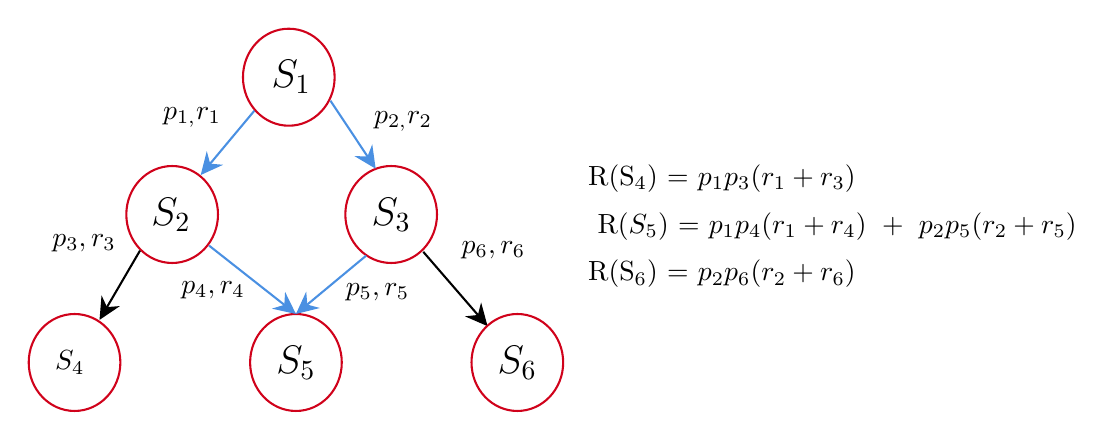
\begin{tikzpicture}[x=0.75pt,y=0.75pt,yscale=-1,xscale=1]
%uncomment if require: \path (0,701.1666717529297); %set diagram left start at 0, and has height of 701.1666717529297

%Straight Lines [id:da8481931635460052] 
\draw    (237.61,125.34) -- (266.62,158.87) ;
\draw [shift={(268.58,161.14)}, rotate = 229.14] [fill={rgb, 255:red, 0; green, 0; blue, 0 }  ][line width=0.08]  [draw opacity=0] (10.72,-5.15) -- (0,0) -- (10.72,5.15) -- (7.12,0) -- cycle    ;

%Shape: Ellipse [id:dp5338816690194331] 
\draw  [color={rgb, 255:red, 208; green, 2; blue, 27 }  ,draw opacity=1 ] (150.73,41.2) .. controls (150.73,28.29) and (160.61,17.83) .. (172.81,17.83) .. controls (185,17.83) and (194.89,28.29) .. (194.89,41.2) .. controls (194.89,54.1) and (185,64.56) .. (172.81,64.56) .. controls (160.61,64.56) and (150.73,54.1) .. (150.73,41.2) -- cycle ;
%Shape: Ellipse [id:dp08323298529021306] 
\draw  [color={rgb, 255:red, 208; green, 2; blue, 27 }  ,draw opacity=1 ] (94.53,107.34) .. controls (94.53,94.44) and (104.41,83.98) .. (116.61,83.98) .. controls (128.8,83.98) and (138.69,94.44) .. (138.69,107.34) .. controls (138.69,120.24) and (128.8,130.7) .. (116.61,130.7) .. controls (104.41,130.7) and (94.53,120.24) .. (94.53,107.34) -- cycle ;
%Shape: Ellipse [id:dp5782501569753735] 
\draw  [color={rgb, 255:red, 208; green, 2; blue, 27 }  ,draw opacity=1 ] (200.05,107.34) .. controls (200.05,94.44) and (209.94,83.98) .. (222.13,83.98) .. controls (234.32,83.98) and (244.21,94.44) .. (244.21,107.34) .. controls (244.21,120.24) and (234.32,130.7) .. (222.13,130.7) .. controls (209.94,130.7) and (200.05,120.24) .. (200.05,107.34) -- cycle ;
%Shape: Ellipse [id:dp9542564413163499] 
\draw  [color={rgb, 255:red, 208; green, 2; blue, 27 }  ,draw opacity=1 ] (47.5,178.64) .. controls (47.5,165.74) and (57.39,155.28) .. (69.58,155.28) .. controls (81.77,155.28) and (91.66,165.74) .. (91.66,178.64) .. controls (91.66,191.54) and (81.77,202) .. (69.58,202) .. controls (57.39,202) and (47.5,191.54) .. (47.5,178.64) -- cycle ;
%Shape: Ellipse [id:dp5730745954231323] 
\draw  [color={rgb, 255:red, 208; green, 2; blue, 27 }  ,draw opacity=1 ] (154.17,178.64) .. controls (154.17,165.74) and (164.06,155.28) .. (176.25,155.28) .. controls (188.44,155.28) and (198.33,165.74) .. (198.33,178.64) .. controls (198.33,191.54) and (188.44,202) .. (176.25,202) .. controls (164.06,202) and (154.17,191.54) .. (154.17,178.64) -- cycle ;
%Shape: Ellipse [id:dp08303160892055261] 
\draw  [color={rgb, 255:red, 208; green, 2; blue, 27 }  ,draw opacity=1 ] (260.84,178.64) .. controls (260.84,165.74) and (270.73,155.28) .. (282.92,155.28) .. controls (295.11,155.28) and (305,165.74) .. (305,178.64) .. controls (305,191.54) and (295.11,202) .. (282.92,202) .. controls (270.73,202) and (260.84,191.54) .. (260.84,178.64) -- cycle ;
%Straight Lines [id:da4561249701318062] 
\draw    (101.12,124.73) -- (83.14,155.52) ;
\draw [shift={(81.62,158.11)}, rotate = 300.3] [fill={rgb, 255:red, 0; green, 0; blue, 0 }  ][line width=0.08]  [draw opacity=0] (10.72,-5.15) -- (0,0) -- (10.72,5.15) -- (7.12,0) -- cycle    ;

%Straight Lines [id:da9228601228550033] 
\draw [color={rgb, 255:red, 74; green, 144; blue, 226 }  ,draw opacity=1 ]   (156.18,57.38) -- (132.29,86.02) ;
\draw [shift={(130.37,88.32)}, rotate = 309.83000000000004] [fill={rgb, 255:red, 74; green, 144; blue, 226 }  ,fill opacity=1 ][line width=0.08]  [draw opacity=0] (10.72,-5.15) -- (0,0) -- (10.72,5.15) -- (7.12,0) -- cycle    ;

%Straight Lines [id:da9215912823895637] 
\draw [color={rgb, 255:red, 74; green, 144; blue, 226 }  ,draw opacity=1 ]   (192.88,52.52) -- (213.01,82.79) ;
\draw [shift={(214.67,85.29)}, rotate = 236.37] [fill={rgb, 255:red, 74; green, 144; blue, 226 }  ,fill opacity=1 ][line width=0.08]  [draw opacity=0] (10.72,-5.15) -- (0,0) -- (10.72,5.15) -- (7.12,0) -- cycle    ;

%Straight Lines [id:da7144026507506241] 
\draw [color={rgb, 255:red, 74; green, 144; blue, 226 }  ,draw opacity=1 ]   (173.89,153.42) -- (134.38,122.31) ;

\draw [shift={(176.25,155.28)}, rotate = 218.22] [fill={rgb, 255:red, 74; green, 144; blue, 226 }  ,fill opacity=1 ][line width=0.08]  [draw opacity=0] (10.72,-5.15) -- (0,0) -- (10.72,5.15) -- (7.12,0) -- cycle    ;
%Straight Lines [id:da10186496684327384] 
\draw [color={rgb, 255:red, 74; green, 144; blue, 226 }  ,draw opacity=1 ]   (178.56,153.36) -- (210.09,127.16) ;

\draw [shift={(176.25,155.28)}, rotate = 320.28] [fill={rgb, 255:red, 74; green, 144; blue, 226 }  ,fill opacity=1 ][line width=0.08]  [draw opacity=0] (10.72,-5.15) -- (0,0) -- (10.72,5.15) -- (7.12,0) -- cycle    ;

% Text Node
\draw (126.24,60.45) node   [align=left] {$\displaystyle p_{1,} r_{1}$};
% Text Node
\draw (227.86,62.45) node   [align=left] {$\displaystyle p_{2,} r_{2}$};
% Text Node
\draw (74.2,121.01) node   [align=left] {$\displaystyle p_{3} ,r_{3}$};
% Text Node
\draw (136.32,143.95) node   [align=left] {$\displaystyle p_{4} ,r_{4}$};
% Text Node
\draw (215.59,144.73) node   [align=left] {$\displaystyle p_{5} ,r_{5}$};
% Text Node
\draw (271.44,124.44) node   [align=left] {$\displaystyle p_{6} ,r_{6}$};
% Text Node
\draw (67.29,178.64) node   [align=left] {$\displaystyle S_{4}$};
% Text Node
\draw (176.25,178.64) node   [align=left] {{\Large $\displaystyle S_{5}$}};
% Text Node
\draw (282.92,178.64) node   [align=left] {{\Large $\displaystyle S_{6}$}};
% Text Node
\draw (116.03,107.34) node  [font=\Large] [align=left] {$\displaystyle S_{2}$};
% Text Node
\draw (222.13,107.34) node  [font=\Large] [align=left] {$\displaystyle S_{3}$};
% Text Node
\draw (173.96,41.2) node  [font=\Large] [align=left] {$\displaystyle S_{1}$};
% Text Node
\draw (381.5,90) node   {R(S$\displaystyle _{4}$) = $\displaystyle p_{1} p_{3}( r_{1} +r_{3})$};
% Text Node
\draw (437,113) node   {R($\displaystyle S_{5}$) = $\displaystyle p_{1} p_{4}( r_{1} +r_{4}) \ +\ p_{2} p_{5}( r_{2} +r_{5})$};
% Text Node
\draw (381.5,136) node   {R(S$\displaystyle _{6}$) = $\displaystyle p_{2} p_{6}( r_{2} +r_{6})$};


\end{tikzpicture}

    \caption{Computing the reward of each absorbing state}
    \label{fig:absstate_reward}
\end{figure}


The reward of each monitoring node is computed the same way, by summing the weighted reward of each absorbing state containing the node.\\
For example, if $Mo^{S_4} = Mo^{S_6} =\{2,4\}$ and $Mo^{S_5} = \{1,4\}$, then the reward of node 4 is computed as $R(N_4) = R(S_4) + R(S_5) + R(S_6)$. Indeed, node 4 belongs to the monitoring set of every absorbing state.



\textbf{Balanced topology: Scenarios a) and b)\\}
Based on the paths taken by attacks and the ordering of the migration, we categorize the nodes into three categories: source, intermediate and border nodes. Source nodes are the origins of attacks, intermediate nodes are going to be on the path of attacks targeting the border nodes. 
The results are shown in Fig.~\ref{fig:mdp-result-topo1}.
The scenario a) sets the source to node 6, nodes 4 and 5 as intermediate nodes and finally nodes 1,2 and 3 as border nodes.
The scenario b) sets the source to nodes 3 and 6, nodes 1 and 4 as intermediate nodes and nodes 2 and 5 as border nodes.
The first observation is that node 6 is globally the most rewarding node in both cases.
This is explained as it is the source of most of the attacks, and the exfiltrated data are redirected there.
In both scenarios, the importance of nodes is separated according to our categorization. 
This means that the nodes pertaining to the majority of attack paths are the most rewarded.
This observation is reinforced in scenario b) where nodes 4 and 5 are close to attack sources while nodes 1 and 2 are further away.

In both scenarios, the detection rate does not have a significant impact on the importance of nodes, as they remain ranked in the same order.
In scenario a) results are stable from $p=0.6$ where node 6 overcomes node 4 in reward until $p=0.9$. All other nodes remain closely grouped, and no intermediate or border nodes is standing out.
In scenario b) the higher the detection rate the higher the reward of node 3, the second source of attacks.
The steadiness in the evolution of each node shows that the performance of the detection is not a major factor in determining which nodes are best suited for the monitoring. 
% We formulate some hypotheses in Section~\ref{sec:mdp-discussion}.

Detailed examination of the optimal policy for each budget also shows that the monitoring action is rarely used to redeploy resources elsewhere in the infrastructure.
Instead of unmonitoring nodes, the MDP chooses to do nothing to preserve the global detection probability.
Unmonitoring actions are only chosen when the unmonitored node is not on the path of the next attacks, thus having the same impact as doing nothing. 
This situation happens rarely, when the attacker launches a limited number of attacks on the infrastructure.

\textbf{Full-mesh topology: Scenarios c) and d) \\}
In these scenarios, the topology considered is full-meshed, which means that each physical node is connected to every other node of the infrastructure. This topology has been chosen to minimize the impact of the routing on the detection path because the attacker is always connected to the target node.
Results are shown in Fig.~\ref{fig:mdp-result-fullmesh}.

We make two observations from the results of both scenarios.
The first observation is that whether there is one or several attackers, the ranking of nodes based on their individual performance remains constant. This reinforces our conclusion that the routing of attacks has a real impact on the detection performance of each node.
The second observation is that the most important nodes are the main source of attacks as well as the first node being migrated. While the first target is an obvious choice for attack detection, the second target shows another aspect of the model which is target selection. Indeed, since node 1 is always migrated first, it is therefore the main target at the first transition of the MDP.

% Finally, we have examined the different optimal policies for these scenarios, and observed that some corner cases have appeared.
% Overall, the fact that for each attack only the origin of the attack and the target node may contribute to the detection has generated a diverse solution state. Simply put, 

% Each solution is composed of only two nodes. Because of the fullmesh aspect of the topology, it is complex to obtain a solution state 
% Indeed, depending on which node is targeted, there are only two nodes in the solution for the detection of the attack. and the fullmesh aspect of the topology makes it hard for those solution sets to overlap and give a better coverage.

\textbf{Central topology: Scenarios e) and f) \\}
Using the same categorization as scenarios a) and b), we consider node 6 as a source node, node 2 as an intermediate node and nodes 1, 3, 4 and 5 as border nodes. Scenario f) transfers node 1 from a border node to a source node. Results are shown in Fig.~\ref{fig:mdp-result-topo2}.

In scenario e), the importance of each node depicted in Fig.~\ref{fig:mdp-result-topo2} reflects their role. Nodes 1, 3, 4 and 5 do not have much impact in the solution set, as they are not on the path of most of attacks. The attack source is still considered important to monitor and node 2 which acts as a ``bridge" between the two halves of the topology will belong to the path of a lot of attacks.

Scenario f) highlights similar results. There are now two attack sources, nodes 1 and 6. Moreover, the geographical distribution of migrated nodes gives more importance to node 2 which becomes even more present on the attack paths, as shown in Table~\ref{tab:mdp-attack-source}. This scenario is also the only one in which the main source of attacks is not consistently the most important node for the monitoring.

% Optimal policies also have some corner cases with counter intuitive optimal monitoring nodes but those remain marginal considering the solution space. 



\begin{figure}
    \centering
    \captionsetup[subfigure]{labelformat=empty}
\begin{subfigure}{.5\textwidth}
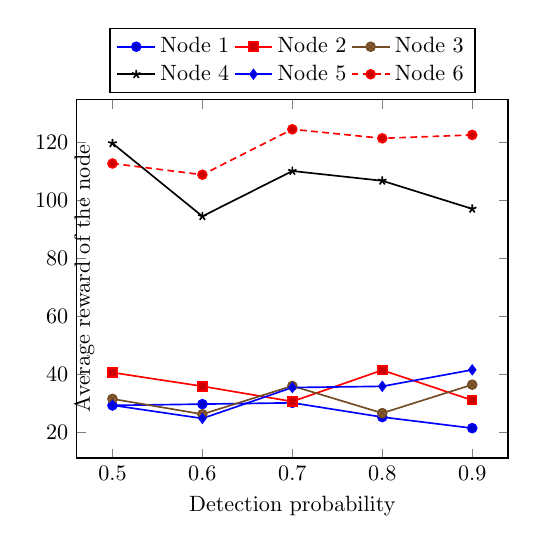
\begin{tikzpicture}[scale=0.8]
\begin{axis}[
  xlabel={Detection probability},
  ylabel={Average reward of the node },
  y label style={at={(0.06,0.5)}},
  xtick={0.5,0.6,0.7,0.8,0.9,1.0},
  legend style={at={(0.5,1.2)},cells={align=right}, anchor=north,legend columns=3},
  grid style=dashed,
]

\addplot+[]
    coordinates {
(0.5,29.2207587022)(0.6,29.6591500811)(0.7,30.107769581)(0.8,25.1808225374)(0.9,21.3501334315)
};

\addplot+[]
    coordinates {
(0.5,40.5649596864)(0.6,35.8317201966)(0.7,30.5615817425)(0.8,41.4017616625)(0.9,31.0018428294)
};

\addplot+[]
    coordinates {
(0.5,31.4601711216)(0.6,26.1715912622)(0.7,35.9427616495)(0.8,26.5488358659)(0.9,36.3780765072)
};

\addplot+[]
    coordinates {
(0.5,119.788927983)(0.6,94.566243579)(0.7,110.212449824)(0.8,106.844518821)(0.9,97.138069126)
};

\addplot+[]
    coordinates {
(0.5,29.2697135288)(0.6,24.7098561839)(0.7,35.3909999115)(0.8,35.8083893589)(0.9,41.5087141375)
};

\addplot+[]
    coordinates {
(0.5,112.808511307)(0.6,108.932780706)(0.7,124.631408718)(0.8,121.507931814)(0.9,122.678991306)
};

\legend{Node 1, Node 2, Node 3, Node 4, Node 5, Node 6}
\end{axis}
\end{tikzpicture}

\caption{Scenario a)}
\label{fig:nodeimp_single}
\end{subfigure}
\begin{subfigure}{.33\textwidth}
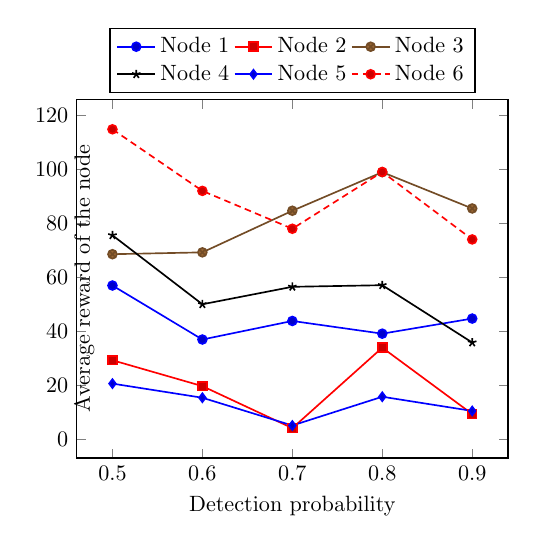
\begin{tikzpicture}[scale=0.8]
\begin{axis}[
  xlabel={Detection probability},
  ylabel={Average reward of the node },
  y label style={at={(0.06,0.5)}},
  xtick={0.5,0.6,0.7,0.8,0.9,1.0},
  legend style={at={(0.5,1.2)},cells={align=right}, anchor=north,legend columns=3},
  grid style=dashed,
]

\addplot+[]
    coordinates {
(0.5,57.0711574474)(0.6,37.0782125822)(0.7,43.9471043804)(0.8,39.2446371458)(0.9,44.8363801675)
};

\addplot+[]
    coordinates {
(0.5,29.4097815394)(0.6,19.8278112984)(0.7,4.26428571429)(0.8,34.0706693208)(0.9,9.49928571429)
};

\addplot+[]
    coordinates {
(0.5,68.6596096998)(0.6,69.339332514)(0.7,84.7438538657)(0.8,99.0264041517)(0.9,85.5894326243)
};

\addplot+[]
    coordinates {
(0.5,75.6609039908)(0.6,50.1243516403)(0.7,56.5923700845)(0.8,57.1874277411)(0.9,35.9649500717)
};

\addplot+[]
    coordinates {
(0.5,20.7573450249)(0.6,15.5267400966)(0.7,5.25375523139)(0.8,15.8992854434)(0.9,10.6415647894)
};

\addplot+[]
    coordinates {
(0.5,114.89762846)(0.6,92.0949728442)(0.7,78.0795310037)(0.8,99.102629324)(0.9,74.1266846482)
};

\legend{Node 1, Node 2, Node 3, Node 4, Node 5, Node 6}
\end{axis}
\end{tikzpicture}

\caption{Scenario b)}
\label{fig:nodeimp_topo1_multiple}
\end{subfigure}
    \caption{Results for single and multiple attackers}
    \label{fig:mdp-result-topo1}
\end{figure}
\begin{figure}
    \centering
    \captionsetup[subfigure]{labelformat=empty}
\begin{subfigure}{.5\textwidth}
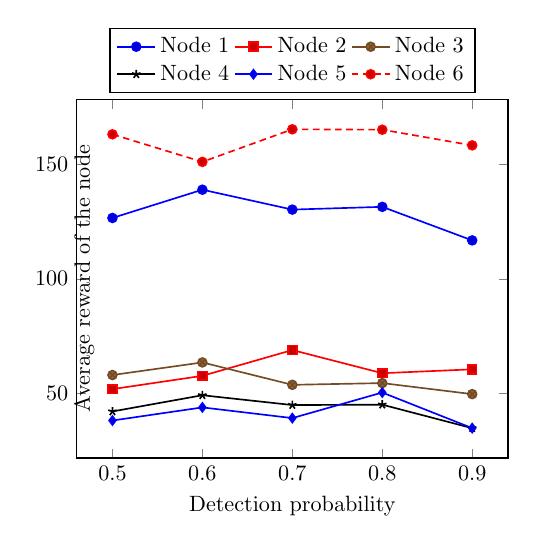
\begin{tikzpicture}[scale=0.8]
\begin{axis}[
  xlabel={Detection probability},
  ylabel={Average reward of the node },
  y label style={at={(0.06,0.5)}},
  xtick={0.5,0.6,0.7,0.8,0.9,1.0},
  legend style={at={(0.5,1.2)},cells={align=right}, anchor=north,legend columns=3},
  grid style=dashed,
]

\addplot+[]
    coordinates {
(0.5,126.469294224)(0.6,138.768688772)(0.7,130.10979383)(0.8,131.308647284)(0.9,116.70873472)
};

\addplot+[]
    coordinates {
(0.5,51.9774584454)(0.6,57.7615872131)(0.7,68.9811633084)(0.8,58.9060250618)(0.9,60.5911805552)
};

\addplot+[]
    coordinates {
(0.5,58.112876005)(0.6,63.5894390224)(0.7,53.8483204974)(0.8,54.5969922461)(0.9,49.8027670671)
};

\addplot+[]
    coordinates {
(0.5,42.2594496478)(0.6,49.3133895991)(0.7,45.0502147208)(0.8,45.20918204)(0.9,34.9808016775)
};

\addplot+[]
    coordinates {
(0.5,38.3055097066)(0.6,44.0188235767)(0.7,39.3680288222)(0.8,50.4912779668)(0.9,34.9978557067)
};

\addplot+[]
    coordinates {
(0.5,162.87848727)(0.6,150.876767477)(0.7,165.06110317)(0.8,164.882126918)(0.9,158.067481047)
};

\legend{Node 1, Node 2, Node 3, Node 4, Node 5, Node 6}
\end{axis}
\end{tikzpicture}

\caption{Scenario c)}
\label{fig:nodeimp_topofullmesh_single}
\end{subfigure}
\begin{subfigure}{.33\textwidth}
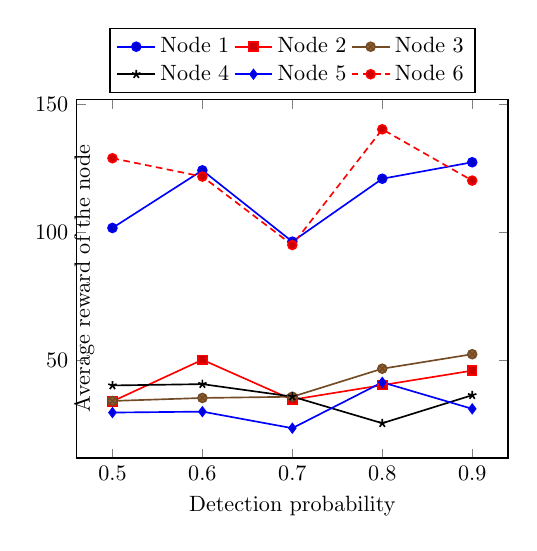
\begin{tikzpicture}[scale=0.8]
\begin{axis}[
  xlabel={Detection probability},
  ylabel={Average reward of the node },
  y label style={at={(0.06,0.5)}},
  xtick={0.5,0.6,0.7,0.8,0.9,1.0},
  legend style={at={(0.5,1.2)},cells={align=right}, anchor=north,legend columns=3},
  grid style=dashed,
]
\addplot+[]
    coordinates {
(0.5,101.616873023)(0.6,124.145242333)(0.7,96.2616914651)(0.8,120.862819291)(0.9,127.305784272)
};

\addplot+[]
    coordinates {
(0.5,33.8037034841)(0.6,50.0693289402)(0.7,34.460597311)(0.8,40.1535742549)(0.9,45.8166364524)
};

\addplot+[]
    coordinates {
(0.5,33.9581528218)(0.6,35.1326808601)(0.7,35.6074089582)(0.8,46.5769811834)(0.9,52.2400544067)
};

\addplot+[]
    coordinates {
(0.5,40.0224063598)(0.6,40.5434953331)(0.7,35.6681036149)(0.8,25.2556265302)(0.9,36.2111392677)
};

\addplot+[]
    coordinates {
(0.5,29.4251886633)(0.6,29.7859232959)(0.7,23.3183642626)(0.8,41.2471235042)(0.9,30.8838558151)
};

\addplot+[]
    coordinates {
(0.5,128.882560148)(0.6,121.704109507)(0.7,94.9489538016)(0.8,140.19719198)(0.9,120.142225907)
};


\legend{Node 1, Node 2, Node 3, Node 4, Node 5, Node 6}
\end{axis}
\end{tikzpicture}

\caption{Scenario d)}
\label{fig:nodeimp_topofullmesh_multiple}
\end{subfigure}
\caption{Results for single and multiple attackers - Scenarios c) and d)}
    \label{fig:mdp-result-fullmesh}
\end{figure}
\begin{figure}
    \centering
    \captionsetup[subfigure]{labelformat=empty}
\begin{subfigure}{.5\textwidth}
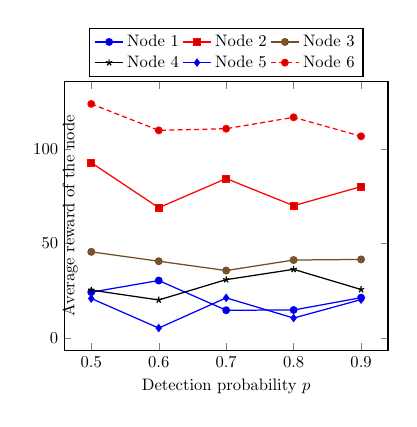
\begin{tikzpicture}[scale=0.6]
\begin{axis}[
  xlabel={Detection probability $p$},
  ylabel={Average reward of the node },
  y label style={at={(0.06,0.5)}},
  xtick={0.5,0.6,0.7,0.8,0.9,1.0},
  legend style={at={(0.5,1.2)},cells={align=right}, anchor=north,legend columns=3},
  grid style=dashed,
]
\addplot+[]
    coordinates {
(0.5,24.2596903238)(0.6,30.4098004181)(0.7,14.7157392372)(0.8,14.8410159329)(0.9,21.3512325325)
};

\addplot+[]
    coordinates {
(0.5,92.6967638225)(0.6,68.892572501)(0.7,84.3050837463)(0.8,69.9668923619)(0.9,80.051680541)
};

\addplot+[]
    coordinates {
(0.5,45.5695982478)(0.6,40.6246377658)(0.7,35.692885081)(0.8,41.2436256503)(0.9,41.5670235599)
};

\addplot+[]
    coordinates {
(0.5,25.3670893308)(0.6,20.1438895136)(0.7,30.888009803)(0.8,36.3312849347)(0.9,25.6728772368)
};

\addplot+[]
    coordinates {
(0.5,20.9174008986)(0.6,5.30161144168)(0.7,21.2602459651)(0.8,10.5837610733)(0.9,20.3331330431)
};

\addplot+[]
    coordinates {
(0.5,123.776293271)(0.6,109.788318837)(0.7,110.653974948)(0.8,116.685625909)(0.9,106.649803871)
};

\legend{Node 1, Node 2, Node 3, Node 4, Node 5, Node 6}
\end{axis}
\end{tikzpicture}

\caption{Scenario e)}
\label{fig:nodeimp_topo2_single}
\end{subfigure}
\begin{subfigure}{.33\textwidth}
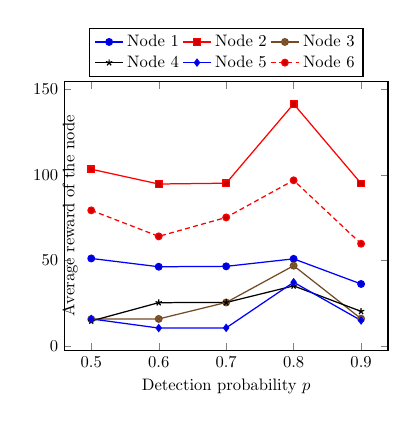
\begin{tikzpicture}[scale=0.6]
\begin{axis}[
  xlabel={Detection probability $p$},
  ylabel={Average reward of the node },
  y label style={at={(0.06,0.5)}},
  xtick={0.5,0.6,0.7,0.8,0.9,1.0},
  legend style={at={(0.5,1.2)},cells={align=right}, anchor=north,legend columns=3},
  grid style=dashed,
]

\addplot+[]
    coordinates {
(0.5,51.2408756424)(0.6,46.3989088055)(0.7,46.629281859)(0.8,51.0165854846)(0.9,36.3262102772)
};

\addplot+[]
    coordinates {
(0.5,103.390154828)(0.6,94.7445634867)(0.7,95.2136135648)(0.8,141.564157095)(0.9,95.0544799628)
};

\addplot+[]
    coordinates {
(0.5,15.7876437463)(0.6,15.9058652472)(0.7,25.5235856726)(0.8,47.0026051031)(0.9,16.0455657836)
};

\addplot+[]
    coordinates {
(0.5,14.6911918445)(0.6,25.4076999562)(0.7,25.5090975344)(0.8,35.2122191081)(0.9,20.3233753667)
};

\addplot+[]
    coordinates {
(0.5,15.9163072098)(0.6,10.573393829)(0.7,10.6704256682)(0.8,37.3424358141)(0.9,14.9838488261)
};

\addplot+[]
    coordinates {
(0.5,79.3520830459)(0.6,64.1507914239)(0.7,75.2190374666)(0.8,96.912552594)(0.9,59.8478399229)
};

\legend{Node 1, Node 2, Node 3, Node 4, Node 5, Node 6}
\end{axis}
\end{tikzpicture}

\caption{Scenario f)}
\label{fig:nodeimp_topo2_multiple}
\end{subfigure}
\caption{Results for single and multiple attackers - Scenarios e) and f)}
    \label{fig:mdp-result-topo2}
\end{figure}

